%!TEX root = ../Project.tex

\section{Implementation}

\subsection{Overview}

\begin{figure}[htbp]
	\centering
		% TODO fix labels
		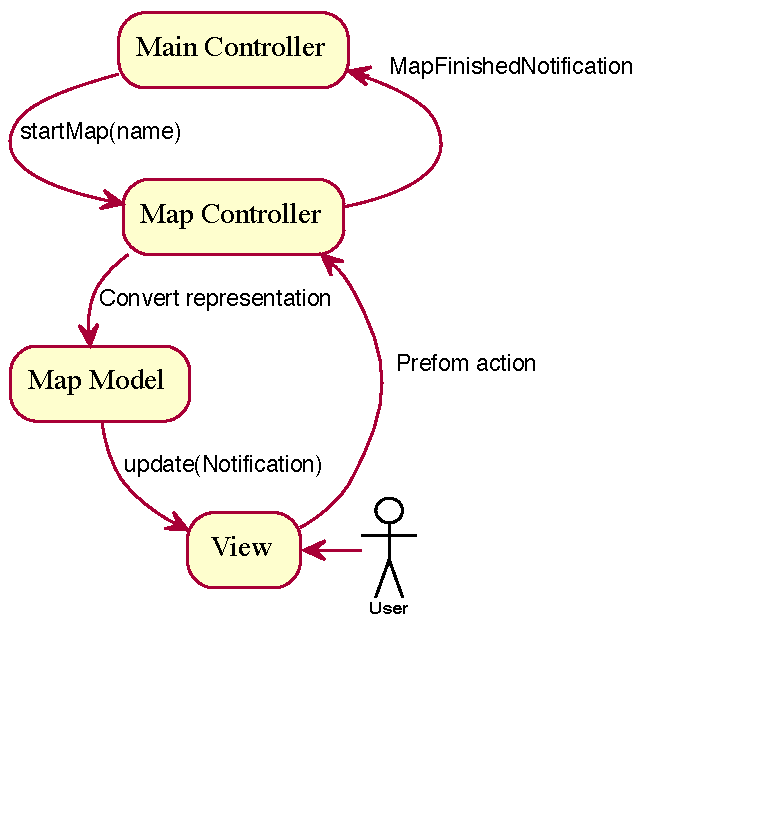
\includegraphics{figures/engine_exported.pdf}
	\caption{Overview of the implementation.}
	\label{fig:overview_engine}
\end{figure}

The system is structures using MVC for the overall architecture as well as  using the Observer Patten as shown above.
%TODO explain  mvc and Observer Patten somewhere

The \texttt{MainController} handles the overall logic, including the game progression. 
Although the objectives only required a isometric  map view, the implementation was designed to be more general  hence a \emph{separate} controller for each \texttt{stage} of the game is used. When the \texttt{stage} is  (e.g. when a map has been completed) the controller notifies the \texttt{MainController}, which decides what to do next.   

%TODO where to put this
%The architecture could be easily extended to overworld maps, cut-scenes for example.


The obsverable components (i.e the view, or the map controller) communicate using \texttt{notification} objects which encapsulates any relevant information. For example the \texttt{model} sends a \texttt{UnitMovedNotification} when the computer controlled opponent move one of their units. The notification includes a reference to the unit moved and the path it took to to get there. This information is used to display an animation of the unit moving to the user.

\clearpage
\subsection{Data Format}
The schema for the data format was only slightly changed for the reason stated in section \ref{ssub:intercompatibility}. To parse and serialisation the xml  the \texttt{Xstream} Java library was used.

XStream is an open source library used to serialise Java objects to and from XML. One of the it major benefits it that it abstracts over the parsing and serialisation and allows the user to focus on what the data should be used for. 

XStream achieves this though the use of Java annotations\footnote{A special form of syntactic metadata that can be added to source of a Java file, with the notable feature of being retained in the complied class files.	}, as shown in the below example\footnote{Getter, Setters and trivial constructor omitted.}.

\begin{lstlisting}[caption=Example of class that is serialisable with XStream, label=lst:SavedTile, language=java] %Java
	
@XStreamAlias("tile")
public class SavedTile {
	protected final String type;
	protected final int height; 
	protected int startingHeight;
	
	@XStreamAsAttribute
	protected final int x;
	@XStreamAsAttribute
	protected final int y;

	protected Orientation orientation;
	protected String leftWall, rightWall;
	
	private Object readResolve() {
		if (orientation == null)  
			orientation = Orientation.TO_EAST;
		if (startingHeight == 0 && height != 0) startingHeight = height;
		return this;
	}}
\end{lstlisting}
As shown above no extra logic apart from the annotations is need for serialisation.  Another benefit of XStream is that it allows setting default values. This allows the user to omit redonent tags, as shown in the xml where most of the tags have been omitted.
\begin{lst:tile}[caption=Serialised form of the above class. ]
<tile x="0" y="0">
	<type>grass</type>
	<height>1</height>
</tile>
\end{lst:tile}

%TODO Ref

\subsubsection{Resources}

All resources that loaded are \texttt{Identifiable}, that they have a unique id.  There are two main advantage to using this scheme. The first is that it allows caching of resources which means that there's single instance for each resource (such as weapons and images). This is especially important for the images, to reduce the memory requirements as well as the load times.

The other advantage is that it meant I could use the same framework for loading and saving all the resources, hence saving development time as well as reducing code duplication. 

A detail description of the structure and  required resource of a project is in appendix \ref{sec:project_structure___specification}.

\subsubsection{Sprite Sheets}
\label{ssub:sprite_sheets}


A sprite sheet is a collection of images combined together. The advantage of this is that a single image is loaded, which reduces loading times. It also make it easier to cache images, since a \emph{subimage} can be efficient created\footnote{using the Java method \texttt{BufferedImage.getSubimage}}. A \texttt{subimage} shares the same image data as original so is ideal way for each tile to have access to it's images\cite{bufferedImage}.    

\begin{figure}[htbp]
	\centering
		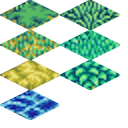
\includegraphics{figures/tileset.png}
	\caption{A 128\*128 sprite sheet containing a tileset for a map}
	\label{fig:figures_tileset}
\end{figure}

Sprite sheets make maps more reusable, since the tileset can be changed without any constiance\footnote{As long as the new tileset has the same number of image or the \texttt{tilemapping} has entires for missing images.}.  

I created a sprite sheet editor to allow the user to easily edit the tilesets. Using sprite sheets allows abstracting over the file system, hence increasing the usability of system. The editor was reused for editing other images such as the character images and can even be used interpedently.
%TODO real word?

\clearpage
\subsection{Engine Development and Testing}
\label{sub:engine_development_and_testing}
\subsubsection{Map}
\label{ssub:maps}

% \begin{itemize}
% 	\item Handles loading
% 	\item Handles events
% 	\item Send messages
% \end{itemize}

The \texttt{Map} class handles the overall logic and game flow.   The main components are:
\begin{itemize}
\item The tiles for the maps. Each tile includes height information as well as the tile's location, as shown in listing \ref{lst:SavedTile}.

\item The enemy unit.     

\item The \texttt{TileMapping} which specify what images to use when draw the images in addition to \emph{how} the tile is drawn. 

\item  The \texttt{conditions} of the maps. These include a winning conditions (such as ``Defeat all Enemy units'',  the placement of player's units and a \texttt{turnComparator} which decides how the turn ordering works.  

\item  The \texttt{events}. These include the dialog which displays parts of the story at the start and end of each dialog. 
\end{itemize}

The other major responsibly of the map is to send notifications to the view.  

\subsubsection{Units}
\label{ssub:units}
A \texttt{unit} has set of attributes whose values can be specified by the user. A unit is the abstract replaction and is storage.  A \texttt{MapUnit} extends the units sets of attributes with extra information such the location and the current hit points.

A unit has a  specified weapon (as discussed in section \ref{sub:weapons___skills}).  A weapon has a \emph{attack range} which specified how the unit attacks.  As a example consider a spear which attacks all units in a specified direction and a bow which attack a single faraway target. A unit with same attributes would  play very differently with either of examples since a spear can be only used in melee combat, whereas a bow can only be used from a distances.

\begin{itemize}
	\item Has a set number of attributes inuldes weapons, images
	\item behaviour for the ai.  
\end{itemize}

\subsubsection{Conditions}
\label{ssub:events}

\begin{itemize}
	\item win conditions.
\end{itemize}

\subsubsection{Algorithms}
\label{ssub:Algorithms}

\begin{itemize}
	\item Unit movement
	\item path finding
	\item AI behaviour
\end{itemize}


\subsubsection{Dialog}
\label{ssub:dialog}
The engine supports displays dialog to the user at the start and end of a battle.

\begin{figure}[htbp]
	\centering
		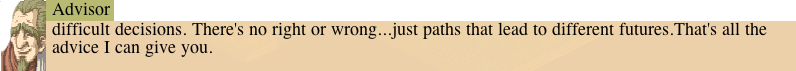
\includegraphics[width=6.3in]{figures/dialog2.png}
	\caption{A example of a dialog}
	\label{fig:figures_dialog2}
\end{figure}

One of the major features is that is that the engine handles line wrapping and pagination of the text which is in contrast to many earlier games. This allows the user to focus on writes the plot of game rather then on fitting the text into the dialog box. 

Optionally a speaker can be specified for the dialog, this can be used to have a conversation between characters on a map, to make the dialog more intertavage. 

The editor as discussed in section \ref{ssub:dialog_editing} supports editing of the dialog. It has the notable features of allowing the user to visually reorder parts of the dialog. It also supports for  importing and exporting the dialog as a text file.  This allows the user to write the script of the game inderpendetry in whatever application they prefer. 


\subsection{Saving and Loading}
The engine supports Saving and Loading at any point during the game. The only possible downside  for the user is that when the the saved data is loaded, game continues from the beginning of the map which was lasted played. 

The reason for this limitation is to keep the save format small and easy to load. sUsing this methods means the only details that need to be saved are the maps left to be played and units attributes (which can change since units can `level up'). 

The other limitation is that there only one save file. This not as big limitation as it seems since the the save file is stored in users home directory, meaning each user would have their own save.

\subsubsection{Inter-compatibility}
\label{ssub:intercompatibility}
As discussed previously the maps use xml as their data format, one the advantages of this was that it required very little changes to the data format to have incompatibility with Oleksandr Stasyk's  Terrain Generator's output format.  The Terrain generator allows uses various algorithms to produce senabient looking map. Users can use these as a starting point, to make it for them to design their maps.

The terrain generator is called by the editor on behalf on the user with appropriate settings saving the user from having to configure the many options  available in the terrain generator.

\subsection{Gui Development and Testing}

\subsubsection{Map Rendering}
\label{ssub:map_rendering}

\begin{itemize}
	\item Isometric maths
	\item how reusable it is
	\item efficient 
\end{itemize}

\subsection{User Interface}

\begin{itemize}
	\item unit animations
	\item menus
\end{itemize}

\subsubsection{Custom Classes} % allows user to use their own code
\label{ssub:custom_classes}


\subsection{Editor Development and Testing}

\subsubsection{Overview}
\label{ssub:overview}

\subsubsection{Map Editor}
\label{ssub:map_editor}

\subsubsection{Unit Editor}
\label{ssub:unit_editors}

\clearpage
\subsubsection{Dialog Editing}
\label{ssub:dialog_editing}

\begin{figure}[htbp]
	\centering
		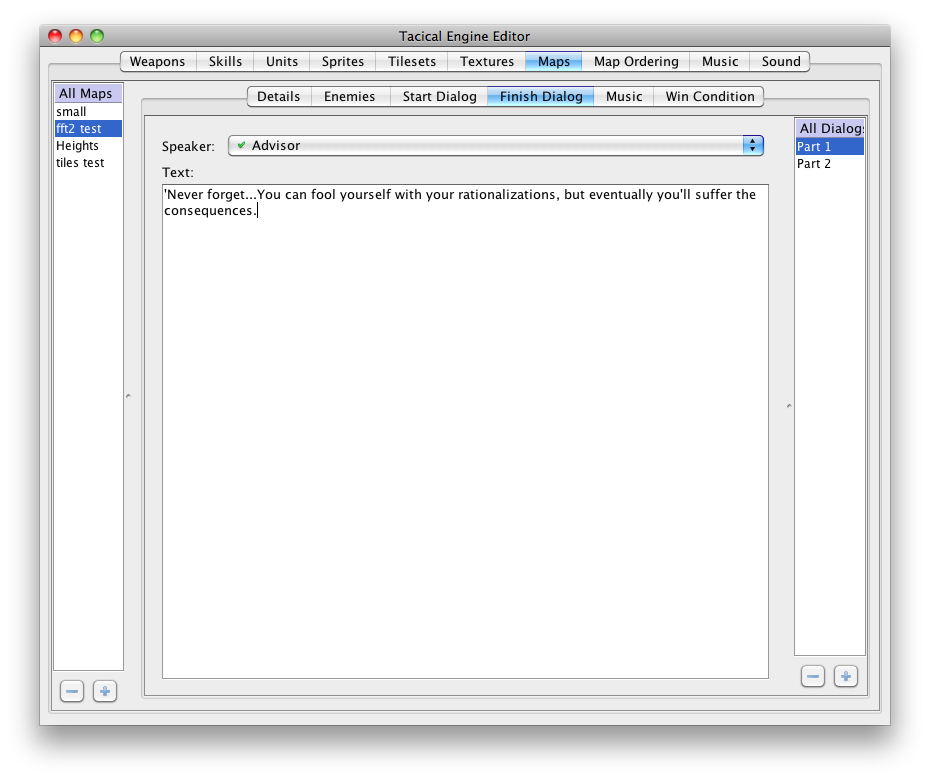
\includegraphics[height=4in]{figures/editor/Maps-dialog.png}
	\caption{The dialog editing panel}
	\label{fig:figures_editor_Maps-dialog}
\end{figure}
The editor supports the creation of dialog.  A dialog is sequaual of parts. Each part has the text  associated with it as well optionally have a speaker.  The speaker can be selected from any unit that is already been placed on the map. This a vast improvement on the original design where the user types the name of the speaker since less change of making errors. \footnote{It would also cause runtime exceptions if there was no unit with that name.}.

As mentioned before, the engine takes care of pagination as well line wrapping when displaying the dialog in the game. This frees the user from having to fit the text into a specified area. 

\paragraph{Import/Export\\}
The editor also supports importing as well as exporting the dialog in format shown below. 
\begin{lstlisting}[caption=Shows the format used  for the dialog]
- speaker1: Some text 
- speaker2: Some more text
- none:     This part has no speaker
\end{lstlisting}
This allows the dialog to be easily written in the user's preferred application.  This could be useful if separate person writes the dialog of the game since the person does not need a copy of the editor. The format is described in more detail in appendix \ref{ssub:dialog_data_format}  


%TODO put bug when loading music stops
\clearpage
\subsubsection{Exporting}
\label{ssub:exporting}

The editor can export the game as a complete package, either as a Mac OS X application or as jar. These application don't require any external resources, apart from a recent version of java\footnote{specifically Java 1.6+}.

A prominent feature of the editor is that the jar will work on any Java enabled platform, since the jar contains all required libraries for each platform. The OS X application can even be exported on other platforms.

While most of the testing was done on OS X \footnote{Mac OS X 10.6 Snow leopard}, it also works well on Linux \footnote{Science  Linux x.y}. It even has limited compatibly with Windows\footnote{Tested on Windows 7 32 bit} (apart from some minor graphics issues).
